\documentclass[12pt]{article}

%------------- PREAMBLE -------------
\usepackage[margin=1in]{geometry}
\usepackage{amsmath,amssymb,mathtools}
\usepackage{enumitem}
\usepackage{bm}
\usepackage{hyperref}
\usepackage{fancyhdr}
\usepackage{draftwatermark}
\usepackage{xcolor}
\usepackage{titlesec}
\usepackage{tikz}
\usetikzlibrary{arrows.meta,calc,positioning}

%------------- TITLE AND METADATA -------------
\newcommand{\CourseCode}{MH1301}
\newcommand{\CourseName}{Discrete Mathematics}
\newcommand{\DocType}{Tutorial 12}

\title{
\CourseCode\ \CourseName \\[0.3em]
\large \DocType
}
\author{
  Academic Year 2025/2026, Semester 2 \\[0.25em]
  \textit{Quantitative Research Society @NTU}
}
\date{\today}

%------------- HEADER & FOOTER (for page 2 onward) -------------
\fancypagestyle{main}{
  \fancyhf{}
  \fancyhead[L]{\CourseCode\ \CourseName}
  \fancyhead[R]{\href{https://qrsntu.org}{QRS@NTU}}
  \fancyfoot[C]{\thepage}
  \renewcommand{\headrulewidth}{0.4pt}
  \renewcommand{\footrulewidth}{0pt}
}

%------------- SIMPLE FOOTER (page 1 only) -------------
\fancypagestyle{plainfirst}{
  \fancyhf{}
  \renewcommand{\headrulewidth}{0pt}
  \renewcommand{\footrulewidth}{0pt}
  \fancyfoot[C]{\scriptsize\textcolor{gray}{\textit{For academic reference only. This document is provided for educational purposes and does not constitute an official question paper, answer key, or any formally authorised academic material. Its content is not guaranteed to be complete or accurate.}}}
}

%------------- WATERMARK -------------
\SetWatermarkText{Unofficial --- QRS@NTU --- qrsntu.org}
\SetWatermarkScale{1}
\SetWatermarkLightness{0.985}

%------------- SHORTCUTS -------------
\newcommand{\N}{\mathbb{N}}
\newcommand{\Z}{\mathbb{Z}}
\newcommand{\R}{\mathbb{R}}
\newcommand{\comp}[1]{\overline{#1}}
\newcommand{\V}{V}
\newcommand{\E}{E}
\newcommand{\degG}{\deg}
\newcommand{\diam}{\operatorname{diam}}

\DeclareMathOperator{\dist}{dist}

\tikzset{
  vtx/.style={circle, draw, minimum size=20pt, inner sep=1pt},
  dotv/.style={circle, fill, inner sep=1.4pt},
  every picture/.style={line cap=round, line join=round}
}

\setcounter{secnumdepth}{-1}
\setcounter{tocdepth}{3}
\setlist[enumerate]{itemsep=0.3em, topsep=0.3em}
\setlist[itemize]{itemsep=0.2em, topsep=0.2em}
\setlength{\headheight}{14.5pt}

\begin{document}

%------------- COVER PAGE -------------
\maketitle
\thispagestyle{plainfirst}
\pagestyle{main}

%====================================================
% OVERVIEW
%====================================================
\begin{center}
  \rule{0.82\textwidth}{0.4pt}\\[4pt]
  \textbf{Overview}\\[2pt]
  \rule{0.82\textwidth}{0.4pt}
\end{center}

\noindent
This tutorial focuses on weighted graphs, minimum spanning trees, shortest paths, and bottleneck spanning trees. The main themes are:
\begin{itemize}[leftmargin=*]
  \item Prim's algorithm and Kruskal's algorithm for minimum spanning trees;
  \item edge-order and cut/cycle reasoning in MST construction;
  \item Dijkstra's algorithm for shortest paths in positively weighted graphs;
  \item shortest-path subpath properties;
  \item minimum bottleneck spanning trees versus minimum spanning trees;
  \item MST cut-property proofs;
  \item explicit MST computation in a complete graph with structured edge weights.
\end{itemize}

\noindent
\textbf{Question map.}
\begin{itemize}[leftmargin=*]
  \item Questions 1--2: Prim's and Kruskal's algorithms on the same weighted graph.
  \item Question 3: MSTs for two separate weighted graphs using different algorithms.
  \item Questions 4--5: Dijkstra's algorithm and shortest-path distances.
  \item Questions 6--7: minimum bottleneck spanning trees and MSTs.
  \item Question 8: Kruskal's algorithm on $K_n$ with edge weights $w(\{u,v\})=u+v$.
\end{itemize}

\newpage
\tableofcontents

%====================================================
% QUESTION 1
%====================================================
\newpage
\section{Question 1 (Prim's algorithm for a minimum spanning tree)}

\subsection{Problem}
\textbf{(Ex. 11.5.2).} Use Prim's algorithm to find a minimum spanning tree for the given weighted graph.

\begin{center}
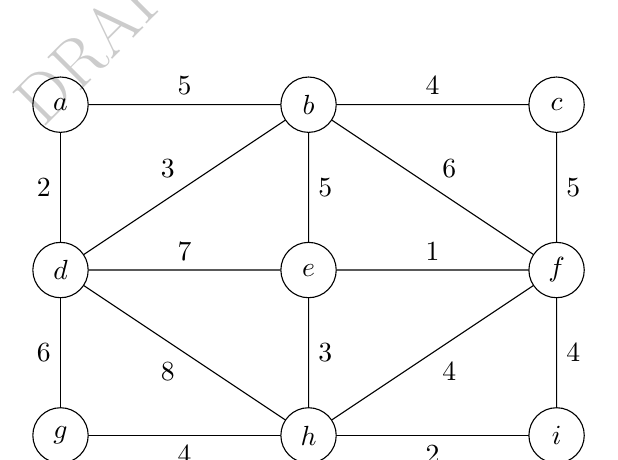
\begin{tikzpicture}[scale=1.05]
  \node[vtx] (a) at (0,4) {$a$};
  \node[vtx] (b) at (3,4) {$b$};
  \node[vtx] (c) at (6,4) {$c$};

  \node[vtx] (d) at (0,2) {$d$};
  \node[vtx] (e) at (3,2) {$e$};
  \node[vtx] (f) at (6,2) {$f$};

  \node[vtx] (g) at (0,0) {$g$};
  \node[vtx] (h) at (3,0) {$h$};
  \node[vtx] (i) at (6,0) {$i$};

  \draw (a)--node[above] {$5$} (b);
  \draw (b)--node[above] {$4$} (c);

  \draw (a)--node[left] {$2$} (d);
  \draw (d)--node[left] {$6$} (g);

  \draw (b)--node[right] {$5$} (e);
  \draw (e)--node[right] {$3$} (h);

  \draw (c)--node[right] {$5$} (f);
  \draw (f)--node[right] {$4$} (i);

  \draw (d)--node[above] {$7$} (e);
  \draw (e)--node[above] {$1$} (f);

  \draw (g)--node[below] {$4$} (h);
  \draw (h)--node[below] {$2$} (i);

  \draw (d)--node[above left] {$3$} (b);
  \draw (b)--node[above right] {$6$} (f);
  \draw (d)--node[below left] {$8$} (h);
  \draw (h)--node[below right] {$4$} (f);
\end{tikzpicture}
\end{center}

\subsection{Solution}

\subsubsection{Method 1: Prim's algorithm starting at $a$}
\textbf{Algorithm used.} Prim's algorithm starts with one vertex and repeatedly adds the minimum-weight edge joining the current tree to a vertex outside it.

Start at vertex $a$.

\[
\begin{array}{c|c|c}
\text{Step} & \text{Current vertex set} & \text{Edge added} \\ \hline
0 & \{a\} & -\\
1 & \{a,d\} & \{a,d\},\ w=2\\
2 & \{a,d,b\} & \{b,d\},\ w=3\\
3 & \{a,d,b,c\} & \{b,c\},\ w=4\\
4 & \{a,d,b,c,e\} & \{b,e\},\ w=5\\
5 & \{a,d,b,c,e,f\} & \{e,f\},\ w=1\\
6 & \{a,d,b,c,e,f,h\} & \{e,h\},\ w=3\\
7 & \{a,d,b,c,e,f,h,i\} & \{h,i\},\ w=2\\
8 & \{a,d,b,c,e,f,h,i,g\} & \{g,h\},\ w=4
\end{array}
\]

Thus one minimum spanning tree obtained by Prim's algorithm is
\[
  T=\bigl\{
  \{a,d\},\{b,d\},\{b,c\},\{b,e\},
  \{e,f\},\{e,h\},\{h,i\},\{g,h\}
  \bigr\}.
\]
Its total weight is
\[
  2+3+4+5+1+3+2+4=24.
\]
Hence
\[
  \boxed{
  E(T)=\{\{a,d\},\{b,d\},\{b,c\},\{b,e\},\{e,f\},\{e,h\},\{h,i\},\{g,h\}\},
  \quad w(T)=24.}
\]

\subsubsection{Method 2: Cut-property verification of the Prim tree}
\textbf{Theorem/criterion used.} For any cut $(S,V\setminus S)$ in a weighted graph, if an edge crossing the cut has strictly minimum weight among all edges crossing that cut, then it is safe for some MST. Prim's algorithm is correct because each selected edge is a safe edge for the cut determined by the current tree.

The selected edges are checked by the corresponding cuts:
\[
\begin{array}{c|c|c}
S & \text{minimum crossing edge chosen} & \text{weight}\\ \hline
\{a\} & \{a,d\} & 2\\
\{a,d\} & \{b,d\} & 3\\
\{a,d,b\} & \{b,c\} & 4\\
\{a,d,b,c\} & \{b,e\}\text{ or }\{c,f\} & 5\\
\{a,d,b,c,e\} & \{e,f\} & 1\\
\{a,d,b,c,e,f\} & \{e,h\} & 3\\
\{a,d,b,c,e,f,h\} & \{h,i\} & 2\\
\{a,d,b,c,e,f,h,i\} & \{g,h\} & 4
\end{array}
\]
At the fourth step there is a tie: $\{b,e\}$ and $\{c,f\}$ both have weight $5$. Choosing either gives an MST of the same total weight.

Therefore the tree found in Method 1 is a minimum spanning tree:
\[
  \boxed{w(T)=24.}
\]

%====================================================
% QUESTION 2
%====================================================
\newpage
\section{Question 2 (Kruskal's algorithm for a minimum spanning tree)}

\subsection{Problem}
\textbf{(Ex. 11.5.4).} Use Kruskal's algorithm to find a minimum spanning tree for the weighted graph in Question 1.

\subsection{Solution}

\subsubsection{Method 1: Kruskal's algorithm by increasing edge weights}
\textbf{Algorithm used.} Kruskal's algorithm sorts all edges in nondecreasing order of weight and adds an edge exactly when it does not create a cycle.

The edges in increasing order of weight are:
\[
\begin{array}{c|c}
\text{Weight} & \text{Edges}\\ \hline
1 & \{e,f\}\\
2 & \{a,d\},\{h,i\}\\
3 & \{b,d\},\{e,h\}\\
4 & \{b,c\},\{f,i\},\{g,h\},\{f,h\}\\
5 & \{a,b\},\{b,e\},\{c,f\}\\
6 & \{d,g\},\{b,f\}\\
7 & \{d,e\}\\
8 & \{d,h\}
\end{array}
\]

Proceeding by Kruskal's algorithm:
\[
\begin{array}{c|c|c}
\text{Order} & \text{Edge considered} & \text{Action}\\ \hline
1 & \{e,f\} & \text{add}\\
2 & \{a,d\} & \text{add}\\
3 & \{h,i\} & \text{add}\\
4 & \{b,d\} & \text{add}\\
5 & \{e,h\} & \text{add}\\
6 & \{b,c\} & \text{add}\\
7 & \{f,i\} & \text{reject: cycle}\\
8 & \{g,h\} & \text{add}\\
9 & \{f,h\} & \text{reject: cycle}\\
10 & \{a,b\} & \text{reject: cycle}\\
11 & \{b,e\} & \text{add}
\end{array}
\]
After $8$ edges have been added, all $9$ vertices are connected, so the MST is complete.

Thus Kruskal's algorithm gives
\[
  T=\bigl\{
  \{e,f\},\{a,d\},\{h,i\},\{b,d\},\{e,h\},
  \{b,c\},\{g,h\},\{b,e\}
  \bigr\}.
\]
The total weight is
\[
  1+2+2+3+3+4+4+5=24.
\]
Therefore
\[
  \boxed{
  E(T)=\{\{e,f\},\{a,d\},\{h,i\},\{b,d\},\{e,h\},\{b,c\},\{g,h\},\{b,e\}\},
  \quad w(T)=24.}
\]

\subsubsection{Method 2: Cycle-property verification}
\textbf{Theorem/criterion used.} The cycle property says that, in any cycle, an edge of strictly largest weight cannot belong to an MST. Kruskal's algorithm repeatedly avoids forming cycles and therefore keeps only safe edges.

The edges rejected in Method 1 are rejected because they close cycles:
\[
\begin{aligned}
\{f,i\}&\text{ closes }f-e-h-i-f,\\
\{f,h\}&\text{ closes }f-e-h-f,\\
\{a,b\}&\text{ closes }a-d-b-a.
\end{aligned}
\]
The final accepted edge $\{b,e\}$ joins the component containing $a,b,c,d$ to the component containing $e,f,g,h,i$. It may be replaced by $\{c,f\}$, which has the same weight $5$, giving another MST of total weight $24$.

Thus the MST need not be unique, but every tree produced here has minimum total weight
\[
  \boxed{24.}
\]

%====================================================
% QUESTION 3
%====================================================
\newpage
\section{Question 3 (Minimum spanning trees for two weighted graphs)}

\subsection{Problem}
Find a minimum spanning tree for each of the following two graphs. Use a different algorithm for each graph. For each graph, state the name of the algorithm used, and list the edges in the order that they are added to the MST.

\begin{center}
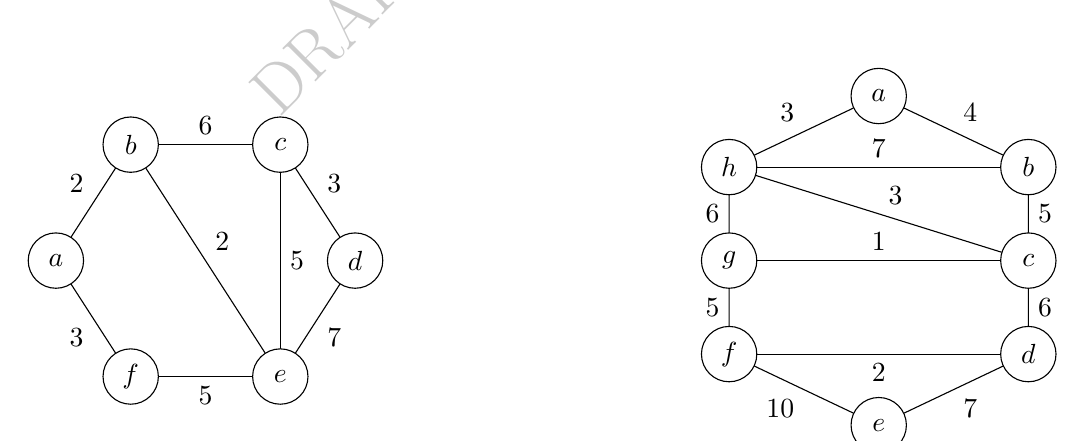
\begin{tikzpicture}[scale=0.95]
  % Left graph
  \begin{scope}[shift={(-4.7,0)}]
    \node[vtx] (a) at (-2,0) {$a$};
    \node[vtx] (b) at (-1,1.55) {$b$};
    \node[vtx] (f) at (-1,-1.55) {$f$};
    \node[vtx] (c) at (1,1.55) {$c$};
    \node[vtx] (e) at (1,-1.55) {$e$};
    \node[vtx] (d) at (2,0) {$d$};

    \draw (a)--node[above left] {$2$} (b);
    \draw (a)--node[below left] {$3$} (f);
    \draw (b)--node[above] {$6$} (c);
    \draw (b)--node[above right] {$2$} (e);
    \draw (c)--node[right] {$5$} (e);
    \draw (c)--node[above right] {$3$} (d);
    \draw (e)--node[below right] {$7$} (d);
    \draw (f)--node[below] {$5$} (e);
  \end{scope}

  % Right graph
  \begin{scope}[shift={(4.3,0)}]
    \node[vtx] (a2) at (0,2.2) {$a$};
    \node[vtx] (h2) at (-2,1.25) {$h$};
    \node[vtx] (b2) at (2,1.25) {$b$};
    \node[vtx] (g2) at (-2,0) {$g$};
    \node[vtx] (c2) at (2,0) {$c$};
    \node[vtx] (f2) at (-2,-1.25) {$f$};
    \node[vtx] (d2) at (2,-1.25) {$d$};
    \node[vtx] (e2) at (0,-2.2) {$e$};

    \draw (h2)--node[above left] {$3$} (a2);
    \draw (a2)--node[above right] {$4$} (b2);
    \draw (h2)--node[above] {$7$} (b2);

    \draw (h2)--node[left] {$6$} (g2);
    \draw (g2)--node[left] {$5$} (f2);

    \draw (b2)--node[right] {$5$} (c2);
    \draw (c2)--node[right] {$6$} (d2);

    \draw (f2)--node[below] {$2$} (d2);
    \draw (g2)--node[above] {$1$} (c2);
    \draw (f2)--node[below left] {$10$} (e2);
    \draw (e2)--node[below right] {$7$} (d2);

    \draw (h2)--node[above right] {$3$} (c2);
  \end{scope}
\end{tikzpicture}
\end{center}

\subsection{Solution}

\subsubsection{Method 1: Prim on the first graph and Kruskal on the second graph}
\begin{enumerate}[label=(\alph*)]
  \item \textbf{First graph: Prim's algorithm starting at $a$.}

  Starting at $a$, add the minimum-weight edge crossing from the current tree to the outside:
  \[
  \begin{array}{c|c|c}
  \text{Step} & \text{Current vertex set} & \text{Edge added}\\ \hline
  0 & \{a\} & -\\
  1 & \{a,b\} & \{a,b\},\ w=2\\
  2 & \{a,b,e\} & \{b,e\},\ w=2\\
  3 & \{a,b,e,f\} & \{a,f\},\ w=3\\
  4 & \{a,b,e,f,c\} & \{e,c\},\ w=5\\
  5 & \{a,b,e,f,c,d\} & \{c,d\},\ w=3
  \end{array}
  \]
  Thus one MST is
  \[
    T_1=\{\{a,b\},\{b,e\},\{a,f\},\{e,c\},\{c,d\}\},
  \]
  with total weight
  \[
    2+2+3+5+3=15.
  \]
  Hence
  \[
    \boxed{E(T_1)=\{\{a,b\},\{b,e\},\{a,f\},\{e,c\},\{c,d\}\},\quad w(T_1)=15.}
  \]

  \item \textbf{Second graph: Kruskal's algorithm.}

  Sort the edges by weight:
  \[
  \begin{array}{c|c}
  \text{Weight} & \text{Edges}\\ \hline
  1 & \{g,c\}\\
  2 & \{f,d\}\\
  3 & \{a,h\},\{h,c\}\\
  4 & \{a,b\}\\
  5 & \{b,c\},\{g,f\}\\
  6 & \{h,g\},\{c,d\}\\
  7 & \{h,b\},\{d,e\}\\
  10 & \{f,e\}
  \end{array}
  \]
  Kruskal's algorithm adds:
  \[
    \{g,c\},\{f,d\},\{a,h\},\{h,c\},\{a,b\},\{g,f\},\{d,e\}.
  \]
  The total weight is
  \[
    1+2+3+3+4+5+7=25.
  \]
  Thus
  \[
    \boxed{
    E(T_2)=\{\{g,c\},\{f,d\},\{a,h\},\{h,c\},\{a,b\},\{g,f\},\{d,e\}\},
    \quad w(T_2)=25.}
  \]
\end{enumerate}

\subsubsection{Method 2: Cut and cycle verification}
\begin{enumerate}[label=(\alph*)]
  \item For the first graph, Prim's chosen edges are safe for the successive cuts
  \[
  \{a\},\quad
  \{a,b\},\quad
  \{a,b,e\},\quad
  \{a,b,e,f\},\quad
  \{a,b,e,f,c\}.
  \]
  The selected crossing edges have weights
  \[
    2,2,3,5,3,
  \]
  respectively. By the cut property, these edges form an MST. Hence
  \[
    \boxed{w(T_1)=15.}
  \]

  \item For the second graph, after adding
  \[
    \{g,c\},\{f,d\},\{a,h\},\{h,c\},\{a,b\},\{g,f\},
  \]
  the only remaining isolated vertex is $e$. The cheaper incident edge to connect $e$ is
  \[
    \{d,e\},\qquad w=7,
  \]
  since
  \[
    w(\{d,e\})=7<10=w(\{f,e\}).
  \]
  The edge $\{b,c\}$ is skipped because it closes the cycle
  \[
    b-a-h-c-b.
  \]
  The edges $\{h,g\}$ and $\{c,d\}$ are skipped because their endpoints are already connected. Therefore Kruskal's accepted edges form an MST of total weight
  \[
    \boxed{25.}
  \]
\end{enumerate}

%====================================================
% QUESTION 4
%====================================================
\newpage
\section{Question 4 (Dijkstra's algorithm from $a$ to $z$)}

\subsection{Problem}
\textbf{(Ex. 10.6.2).} Find the distance between $a$ and $z$ in the following graph using Dijkstra algorithm. Illustrate how the values of $d[v]$ are updated using a table.

\begin{center}
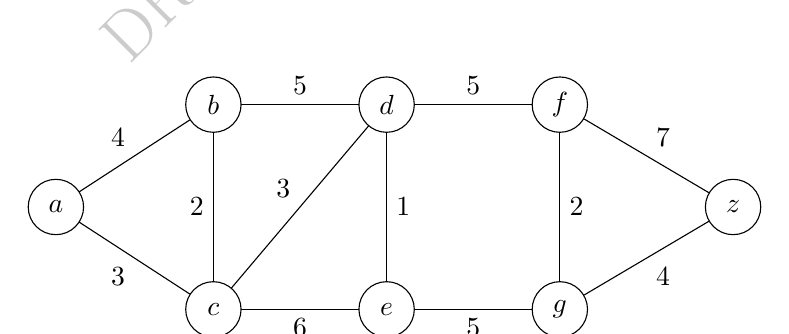
\begin{tikzpicture}[scale=1.0]
  \node[vtx] (a) at (0,0) {$a$};
  \node[vtx] (b) at (2,1.3) {$b$};
  \node[vtx] (c) at (2,-1.3) {$c$};
  \node[vtx] (d) at (4.2,1.3) {$d$};
  \node[vtx] (e) at (4.2,-1.3) {$e$};
  \node[vtx] (f) at (6.4,1.3) {$f$};
  \node[vtx] (g) at (6.4,-1.3) {$g$};
  \node[vtx] (z) at (8.6,0) {$z$};

  \draw (a)--node[above left] {$4$} (b);
  \draw (a)--node[below left] {$3$} (c);
  \draw (b)--node[left] {$2$} (c);
  \draw (b)--node[above] {$5$} (d);
  \draw (c)--node[above left] {$3$} (d);
  \draw (c)--node[below] {$6$} (e);
  \draw (d)--node[right] {$1$} (e);
  \draw (d)--node[above] {$5$} (f);
  \draw (e)--node[below] {$5$} (g);
  \draw (f)--node[right] {$2$} (g);
  \draw (f)--node[above right] {$7$} (z);
  \draw (g)--node[below right] {$4$} (z);
\end{tikzpicture}
\end{center}

\subsection{Solution}

\subsubsection{Method 1: Dijkstra table}
\textbf{Algorithm used.} Dijkstra's algorithm repeatedly selects the unvisited vertex with smallest tentative distance and relaxes all edges incident to it. It is valid here because all edge weights are positive.

The distance labels are updated as follows:
\[
\renewcommand{\arraystretch}{1.25}
\begin{array}{c|cccccccc|l}
\text{Step} & d[a]&d[b]&d[c]&d[d]&d[e]&d[f]&d[g]&d[z] & S\\ \hline
0 & 0&\infty&\infty&\infty&\infty&\infty&\infty&\infty&\varnothing\\
1 & 0&4&3&\infty&\infty&\infty&\infty&\infty&\{a\}\\
2 & 0&4&3&6&9&\infty&\infty&\infty&\{a,c\}\\
3 & 0&4&3&6&9&\infty&\infty&\infty&\{a,c,b\}\\
4 & 0&4&3&6&7&11&\infty&\infty&\{a,c,b,d\}\\
5 & 0&4&3&6&7&11&12&\infty&\{a,c,b,d,e\}\\
6 & 0&4&3&6&7&11&12&18&\{a,c,b,d,e,f\}\\
7 & 0&4&3&6&7&11&12&16&\{a,c,b,d,e,f,g\}\\
8 & 0&4&3&6&7&11&12&16&\{a,c,b,d,e,f,g,z\}
\end{array}
\]
Thus
\[
  d[z]=16.
\]
The shortest path corresponding to the predecessor updates is
\[
  a-c-d-e-g-z,
\]
with total length
\[
  3+3+1+5+4=16.
\]
Therefore
\[
  \boxed{\dist(a,z)=16.}
\]

\subsubsection{Method 2: Shortest-path tree verification}
From Dijkstra's algorithm, the final shortest-path predecessor tree from $a$ is
\[
  \{a c,\ a b,\ c d,\ d e,\ d f,\ e g,\ g z\}.
\]
The corresponding distances are:
\[
\begin{array}{c|cccccccc}
v & a&b&c&d&e&f&g&z\\ \hline
d[v] & 0&4&3&6&7&11&12&16
\end{array}
\]
Each tree edge realizes the displayed distance:
\[
\begin{aligned}
d[c]&=d[a]+3=3,\\
d[b]&=d[a]+4=4,\\
d[d]&=d[c]+3=6,\\
d[e]&=d[d]+1=7,\\
d[f]&=d[d]+5=11,\\
d[g]&=d[e]+5=12,\\
d[z]&=d[g]+4=16.
\end{aligned}
\]
Checking the non-tree edges gives no improvement:
\[
\begin{aligned}
d[b]+2&=6\ge d[c]=3,\\
d[c]+6&=9\ge d[e]=7,\\
d[f]+2&=13\ge d[g]=12,\\
d[f]+7&=18\ge d[z]=16.
\end{aligned}
\]
Hence the labels are final shortest-path distances. Therefore
\[
  \boxed{\dist(a,z)=16.}
\]

%====================================================
% QUESTION 5
%====================================================
\newpage
\section{Question 5 (Shortest path lengths in the graph from Question 4)}

\subsection{Problem}
\textbf{(Ex. 10.6.4).} Find the length of a shortest path between these pairs of vertices in the weighted graph in Question 4.
\begin{enumerate}[label=(\alph*)]
  \item $a$ and $d$;
  \item $a$ and $f$;
  \item $c$ and $f$;
  \item $b$ and $z$.
\end{enumerate}

\subsection{Solution}

\subsubsection{Method 1: Shortest-path tree and local Dijkstra checks}
\begin{enumerate}[label=(\alph*)]
  \item From Question 4, Dijkstra's algorithm gives
  \[
    d[d]=6.
  \]
  A shortest path is
  \[
    a-c-d,
  \]
  with length
  \[
    3+3=6.
  \]
  Hence
  \[
    \boxed{\dist(a,d)=6.}
  \]

  \item From Question 4,
  \[
    d[f]=11.
  \]
  A shortest path is
  \[
    a-c-d-f,
  \]
  with length
  \[
    3+3+5=11.
  \]
  Hence
  \[
    \boxed{\dist(a,f)=11.}
  \]

  \item The path
  \[
    c-d-f
  \]
  has length
  \[
    3+5=8.
  \]
  To verify minimality, run Dijkstra from $c$ until $f$ is settled:
  \[
  \begin{array}{c|cccccccc|l}
  \text{Step} & d[c]&d[b]&d[a]&d[d]&d[e]&d[f]&d[g]&d[z] & S\\ \hline
  0 & 0&\infty&\infty&\infty&\infty&\infty&\infty&\infty&\varnothing\\
  1 & 0&2&3&3&6&\infty&\infty&\infty&\{c\}\\
  2 & 0&2&3&3&6&\infty&\infty&\infty&\{c,b\}\\
  3 & 0&2&3&3&6&\infty&\infty&\infty&\{c,b,a\}\\
  4 & 0&2&3&3&4&8&\infty&\infty&\{c,b,a,d\}\\
  5 & 0&2&3&3&4&8&9&\infty&\{c,b,a,d,e\}\\
  6 & 0&2&3&3&4&8&9&15&\{c,b,a,d,e,f\}
  \end{array}
  \]
  Thus
  \[
    \boxed{\dist(c,f)=8.}
  \]

  \item A shortest path from $b$ to $z$ is
  \[
    b-d-e-g-z,
  \]
  with length
  \[
    5+1+5+4=15.
  \]
  Another shortest path is
  \[
    b-c-d-e-g-z,
  \]
  with length
  \[
    2+3+1+5+4=15.
  \]
  Running Dijkstra from $b$ gives final label $d[z]=15$, so
  \[
    \boxed{\dist(b,z)=15.}
  \]
\end{enumerate}

Thus the requested lengths are
\[
  \boxed{\text{(a) }6,\qquad \text{(b) }11,\qquad \text{(c) }8,\qquad \text{(d) }15.}
\]

\subsubsection{Method 2: Subpath property and reverse-distance check}
\textbf{Theorem/criterion used.} Every subpath of a shortest path is itself a shortest path between its endpoints.

\begin{enumerate}[label=(\alph*)]
  \item Since
  \[
    a-c-d-e-g-z
  \]
  is a shortest path from $a$ to $z$, its subpath
  \[
    a-c-d
  \]
  is a shortest path from $a$ to $d$. Hence
  \[
    \dist(a,d)=3+3=6.
  \]
  Therefore
  \[
    \boxed{\dist(a,d)=6.}
  \]

  \item The Dijkstra shortest-path tree gives the path
  \[
    a-c-d-f.
  \]
  Its length is
  \[
    3+3+5=11.
  \]
  Therefore
  \[
    \boxed{\dist(a,f)=11.}
  \]

  \item The subpath
  \[
    c-d-f
  \]
  of the shortest path
  \[
    a-c-d-f
  \]
  is shortest from $c$ to $f$. Thus
  \[
    \dist(c,f)=3+5=8.
  \]
  Hence
  \[
    \boxed{\dist(c,f)=8.}
  \]

  \item Compute the relevant distances to $z$:
  \[
    \dist(d,z)=1+5+4=10
    \qquad\text{via }d-e-g-z,
  \]
  and
  \[
    \dist(c,z)=3+1+5+4=13
    \qquad\text{via }c-d-e-g-z.
  \]
  Since the neighbours of $b$ are $a,c,d$, any path from $b$ to $z$ must begin with one of
  \[
    b-a,\quad b-c,\quad b-d.
  \]
  Therefore
  \[
  \begin{aligned}
    \dist(b,z)
    &=\min\{4+\dist(a,z),\ 2+\dist(c,z),\ 5+\dist(d,z)\}\\
    &=\min\{4+16,\ 2+13,\ 5+10\}\\
    &=15.
  \end{aligned}
  \]
  Thus
  \[
    \boxed{\dist(b,z)=15.}
  \]
\end{enumerate}

%====================================================
% QUESTION 6
%====================================================
\newpage
\section{Question 6 (Minimum bottleneck spanning trees need not be MSTs)}

\subsection{Problem}
One of the basic motivations behind the Minimum Spanning Tree Problem is the goal of designing a spanning network for a set of nodes with minimum total cost. Here we explore another type of objective: designing a spanning network for which the most expensive edge is as cheap as possible.

Specifically, let $G=(V,E)$ be a connected graph with $n$ vertices, $m$ edges, and positive edge costs that you may assume are all distinct. Let $T=(V,E')$ be a spanning tree of $G$; we define the bottleneck edge of $T$ to be the edge of $T$ with the greatest cost.

A spanning tree $T$ of $G$ is a minimum bottleneck spanning tree if there is no spanning tree $T'$ of $G$ with a cheaper bottleneck edge.

Is every minimum-bottleneck tree of $G$ a minimum spanning tree of $G$? Prove or give a counterexample.

\subsection{Solution}

\subsubsection{Method 1: Explicit counterexample}
The claim is false. Consider the weighted graph
\[
  V=\{a,b,c,d\},
\]
with edge weights
\[
  w(ab)=4,\qquad w(bc)=3,\qquad w(cd)=2,\qquad w(bd)=1.
\]

\begin{center}
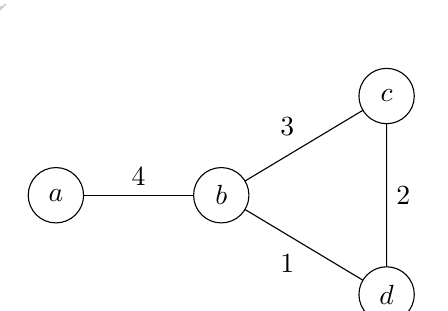
\begin{tikzpicture}[scale=1.05]
  \node[vtx] (a) at (0,0) {$a$};
  \node[vtx] (b) at (2,0) {$b$};
  \node[vtx] (c) at (4,1.2) {$c$};
  \node[vtx] (d) at (4,-1.2) {$d$};

  \draw (a)--node[above] {$4$} (b);
  \draw (b)--node[above left] {$3$} (c);
  \draw (c)--node[right] {$2$} (d);
  \draw (b)--node[below left] {$1$} (d);
\end{tikzpicture}
\end{center}

The vertex $a$ is incident only with the edge $ab$. Hence every spanning tree must contain $ab$, and therefore every spanning tree has bottleneck cost at least
\[
  4.
\]

Now take
\[
  T=\{\{a,b\},\{b,c\},\{c,d\}\}.
\]
This is a spanning tree, and its edge weights are
\[
  4,3,2.
\]
Thus its bottleneck cost is
\[
  4.
\]
Since no spanning tree can have bottleneck cost below $4$, this $T$ is a minimum bottleneck spanning tree.

However, $T$ is not a minimum spanning tree, because
\[
  w(T)=4+3+2=9,
\]
whereas
\[
  T^*=\{\{a,b\},\{b,d\},\{d,c\}\}
\]
has total weight
\[
  w(T^*)=4+1+2=7<9.
\]
Therefore
\[
  \boxed{\text{not every minimum bottleneck spanning tree is a minimum spanning tree}.}
\]

\subsubsection{Method 2: Threshold-connectivity interpretation}
\textbf{Criterion used.} A spanning tree has bottleneck at most $B$ if and only if the subgraph formed by all edges of weight at most $B$ is connected.

In the graph above, the subgraph using only edges of weight at most $3$ has edge set
\[
  \{bd,dc,bc\}.
\]
This subgraph does not contain vertex $a$ as a connected vertex, so it is not connected. Hence no spanning tree has bottleneck at most $3$.

The subgraph using edges of weight at most $4$ is the whole graph and is connected. Therefore the minimum bottleneck value is exactly
\[
  4.
\]
The tree
\[
  \{\{a,b\},\{b,c\},\{c,d\}\}
\]
has bottleneck $4$, so it is minimum-bottleneck. But its total cost is $9$, while the spanning tree
\[
  \{\{a,b\},\{b,d\},\{d,c\}\}
\]
has total cost $7$. Thus the minimum-bottleneck tree need not minimize total weight:
\[
  \boxed{\text{False}.}
\]

%====================================================
% QUESTION 7
%====================================================
\newpage
\section{Question 7 (Every MST is a minimum bottleneck spanning tree)}

\subsection{Problem}
Is every minimum spanning tree of $G$ a minimum-bottleneck tree of $G$? Prove or give a counterexample. \textit{(Hint: use the property of safe edges.)}

\subsection{Solution}

\subsubsection{Method 1: Cut-property proof}
\textbf{Theorem/criterion used.} Let $T$ be an MST. If $e\in E(T)$ and deleting $e$ partitions $T$ into two components with vertex sets $A$ and $B$, then no edge crossing the cut $(A,B)$ has weight smaller than $w(e)$. Otherwise, replacing $e$ by that smaller crossing edge would produce a spanning tree of smaller total weight.

Let $T$ be a minimum spanning tree of $G$. Let $e$ be a bottleneck edge of $T$, so
\[
  w(e)=\max_{f\in E(T)}w(f).
\]
Delete $e$ from $T$. This produces two components with vertex sets $A$ and $B$. Since $T$ is an MST, $e$ is a minimum-weight edge crossing the cut $(A,B)$. Hence every edge crossing the cut has weight at least $w(e)$.

Every spanning tree of $G$ must contain at least one edge crossing the cut $(A,B)$; otherwise it cannot connect vertices in $A$ to vertices in $B$. Therefore every spanning tree has bottleneck edge of weight at least
\[
  w(e).
\]
But $T$ itself has bottleneck weight exactly $w(e)$. Hence no spanning tree has a cheaper bottleneck edge than $T$.

Therefore
\[
  \boxed{\text{every minimum spanning tree is a minimum bottleneck spanning tree}.}
\]

\subsubsection{Method 2: Kruskal-prefix proof}
\textbf{Theorem/criterion used.} Kruskal's algorithm constructs an MST by adding edges in increasing order of weight whenever they connect two different components.

Let $T$ be an MST, and let $B$ be its bottleneck weight. Suppose, for contradiction, that there is a spanning tree $T'$ whose bottleneck is strictly smaller than $B$. Then every edge of $T'$ has weight less than $B$.

Let $e$ be an edge of $T$ with weight $B$. In Kruskal's algorithm, before edges of weight $B$ are used, the graph formed by all edges of weight less than $B$ is not yet connected; otherwise Kruskal would have completed a spanning tree without needing any edge of weight $B$.

But if $T'$ has all edges of weight less than $B$, then the edges of $T'$ form a connected spanning subgraph using only edges of weight less than $B$. This contradicts the fact that the edges of weight less than $B$ do not connect all vertices.

Hence no spanning tree has bottleneck smaller than $B$. Therefore every MST is a minimum bottleneck spanning tree:
\[
  \boxed{\text{True}.}
\]

%====================================================
% QUESTION 8
%====================================================
\newpage
\section{Question 8 (MST of $K_n$ with weights $w(\{u,v\})=u+v$)}

\subsection{Problem}
Let the complete graph $K_n$ have vertices
\[
  \{1,2,\dots,n\}
\]
and suppose that for each
\[
  u,v\in\{1,2,\dots,n\},
\]
the edge $\{u,v\}$ has weight
\[
  w(\{u,v\})=u+v.
\]
For example, edge $\{1,2\}$ has weight $w(\{1,2\})=1+2=3$, edge $\{2,4\}$ has weight $w(\{2,4\})=2+4=6$, etc.

Determine the minimum spanning tree of this graph, and compute the total cost for this minimum spanning tree.

\medskip
\noindent
\textit{Hint: apply Kruskal's algorithm to this graph, and see what are the edges added to the MST.}

\subsection{Solution}

\subsubsection{Method 1: Kruskal's algorithm and cycle rejection}
\textbf{Algorithm used.} Kruskal's algorithm considers edges in nondecreasing order of weight and adds an edge if and only if it does not create a cycle.

We claim that Kruskal's algorithm selects exactly the edges
\[
  \{1,2\},\{1,3\},\dots,\{1,n\}.
\]
These edges form the star centered at $1$.

Consider an edge $\{i,j\}$ with
\[
  2\le i<j\le n.
\]
Its weight is
\[
  w(\{i,j\})=i+j.
\]
The edges
\[
  \{1,i\}
  \qquad\text{and}\qquad
  \{1,j\}
\]
have weights
\[
  1+i<i+j,
  \qquad
  1+j<i+j,
\]
because $i,j\ge 2$. Hence Kruskal's algorithm considers and accepts $\{1,i\}$ and $\{1,j\}$ before it considers $\{i,j\}$.

When $\{i,j\}$ is considered, the vertices $i$ and $j$ are already connected through
\[
  i-1-j.
\]
Thus adding $\{i,j\}$ would create the cycle
\[
  1-i-j-1,
\]
so Kruskal's algorithm rejects it.

Therefore the only accepted edges are
\[
  \{1,2\},\{1,3\},\dots,\{1,n\}.
\]
The total cost is
\[
\begin{aligned}
  \sum_{k=2}^{n} w(\{1,k\})
  &=\sum_{k=2}^{n} (1+k)\\
  &=(n-1)+\sum_{k=2}^{n}k\\
  &=(n-1)+\left(\frac{n(n+1)}{2}-1\right)\\
  &=\frac{n(n+1)}{2}+n-2\\
  &=\frac{(n+1)(n+2)}{2}-3.
\end{aligned}
\]
Hence the MST is
\[
  \boxed{
  E(T)=\{\{1,2\},\{1,3\},\dots,\{1,n\}\},
  \qquad
  w(T)=\frac{(n+1)(n+2)}{2}-3.}
\]

\subsubsection{Method 2: Cut-property proof}
\textbf{Theorem/criterion used.} If an edge is the unique minimum-weight edge crossing a cut, then it belongs to every MST.

For each
\[
  k\in\{2,3,\dots,n\},
\]
consider the cut
\[
  \bigl(\{k\},\{1,2,\dots,n\}\setminus\{k\}\bigr).
\]
The edges crossing this cut are exactly
\[
  \{k,j\}
  \qquad
  (j\neq k).
\]
Their weights are
\[
  w(\{k,j\})=k+j.
\]
This is minimized when
\[
  j=1.
\]
Thus the unique lightest edge crossing the cut is
\[
  \{1,k\},
\]
with weight
\[
  1+k.
\]
By the cut property, every MST contains
\[
  \{1,k\}
  \qquad
  \text{for each }k=2,\dots,n.
\]
There are exactly $n-1$ such edges, and they form a spanning tree. Therefore they are precisely the MST.

Thus
\[
  T=K_{1,n-1}
\]
centered at vertex $1$, and its total cost is
\[
  \sum_{k=2}^{n}(1+k)
  =
  \frac{(n+1)(n+2)}{2}-3.
\]
Therefore
\[
  \boxed{
  \text{the MST is the star centered at }1,\quad
  w(T)=\frac{(n+1)(n+2)}{2}-3.}
\]

\end{document}